\chapter{Tests et analyse défauts fonctionnels ESD}
\label{chap:1}
\section{Contexte}

% What generates an ESD
Une décharge électrostatique est le résultat d'une accumulation de potentiel électrostatique, causée par induction électrique ou de la triboélectricité.
La charge triboélectrique se produit par transfert d'électrons lorsque deux objets sont mis en contact puis séparés.
Un objet se charge positivement et l'autre négativement suivant les matériaux.
La charge par induction se produit lorsque l'objet baigne dans un champs électrique, puis est soudainement mis à la masse.

% Electronic devices are exposed to ESD, in factories first
Les décharges électrostatiques sont un problème important pour les systèmes électroniques.
Des défaillances peuvent se produire pendant la fabrication ou pendant la vie du produit.
Pendant la fabrication, les circuits sont manipulés par des machines, ce qui cause des contacts répétés et éventuellement une accumulation de charges.
Il existe plusieurs standards de test pour garantir qu'un produit peut survivre aux étapes de fabrication.
Les testeurs HMM (Human Machine Model) et CDM (Charged Device Model) valident respectivement la robustesse vis-à-vis de la décharge d'un objet dans le produit, et la décharge du produit dans la masse.
Ces tests sont conçus pour reproduire fidèlement les stress rencontrés dans l'environnement de fabrication.
Généralement, les environnements de fabrication sont appelés EPA (Electrostatic Protected Area) si ils possèdent des équipements qui évitent l'accumulation de charges électrostatiques et autorisent une manipulation des composants électroniques.
Les testeurs HMM et CDM garantissent avant tout que les composants sont capables de survivre à la zone EPA.

% Electronic devices are exposed to ESD in the field
Des défaillances peuvent aussi apparaitre une fois le produit dans son environnement final de fonctionnement.
Dans le cas de produits grand-public et multimédia, elles peuvent être causées par la manipulation des objets par des humains chargés électriquement.
Dans l'environnement automobile, les contraintes sont encore plus fortes à cause d'autres phénomènes de génération de tribo-électricité.

% Hard-failure is one thing, soft-fail another
Il y a deux classes de défaillances dues aux ESD.
La casse matérielle est le premier type de défaillance.
Le composant est détruit après une décharge et doit être remplacé.
La perte de fonctionnalité est le second type de défaillance, et se produit alors que le produit est alimenté et en fonctionnement.
La décharge perturbe une ou plusieurs fonctions, qui a besoin d'un délai pour récupérer.
Parfois, la fonction est bloquée et un redémarrage manuel du produit est requis pour rétablir un fonctionnement normal.
Ce genre de faute est très problématique pour les systèmes temps-réel, censés réagir immédiatement et sans interruption.

\section{Méthodes de test ESD}

Pour reproduire les décharges électrostatiques dans un laboratoire, de multiples générateurs de test existent.
Le TLP (Transmission Line Pulser) est un des plus largement utilisés.
Il est employé dans une variété d'applications, pour la characterization de composants \cite{TLPforESDProtectionCz, TLPthroubleshooting}, l'investigation de défaillances \cite{tlp-application-1, tlp-application-2} et la corrélation avec d'autre générateurs de test \cite{correlation-system-level-esd-tlp}.
Cette technique a été inventée par T. Maloney et N. Nakamura \cite{TLP}.
Elle est standardisée sous la référence ANSI/ESD STM 5.5.1-2016 \cite{tlp-standard}.
Ce type de générateur est détaillé dans les thèses de N. Monnereau \cite{phd-monnereau} et N. Lacrampe \cite{phd-lacrampe}.

% Concept
Un TLP génère une impulsion rectangulaire très courte, en utilisant la décharge d'un câble coaxial (Fig. \ref{tlp_concept}).
Le câble est initialement chargé par une source haute-tension à travers une résistance de forte valeur.
Une fois la tension du câble suffisamment élevée, un relai est commuté pour déclencher la décharge.
Le câble utilisé a généralement une impédance caractéristique de 50\textOmega{} et une longueur de 10 mètres, correspondant à un délai de 50 ns de propagation.
La décharge produite par un tel câble est deux fois plus longue (à cause des effets de propagation) et dure 100 ns.

\begin{figure}[!h]
  \centering
  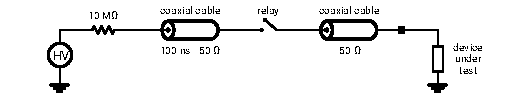
\includegraphics[width=\textwidth]{src/1/figures/tlp_concept.pdf}
  \caption{Configuration minimale d'un générateur TLP}
  \label{tlp_concept}
\end{figure}

% Characteristics of tlp systems
Un système TLP produit des impulsions très reproductibles, car l'environnement est très bien maitrisé et la décharge a lieu dans un chemin de propagation blindé et isolé des perturbations extérieures.
L'impédance caractéristique de 50\textOmega{} peut être maintenue jusqu'à la charge.

% ESD guns
Le TLP est un excellent outil de test et d'investigation, mais la forme d'onde est très différente d'une vraie décharge électrostatique.
Par ailleurs, pour mettre un produit sur le marché il est nécessaire de la qualifier à l'aide des testeurs type "pistolets de décharge ESD".
Ces testeurs ne permettent pas par contre une investigation aussi aisée et poussée que le TLP.
Les standards IEC 61000-4-2 \cite{iec61000-4-2} et ISO 10605 \cite{iso10605} définissent une forme d'onde de qualification pour les systèmes électroniques.
Elle reproduit la décharge d'un corps humain à travers un circuit électronique.
Ces tests sont utilisés très largement pour la qualification des produits.
Un pistolet ESD est constitué d'une pointe métallique qui sert à injecter la décharge.
Le retour de masse est assuré par un câble métallique long de quelques mètres.

% How is the pulse generated
La génération de la décharge est assurée en théorie par une résistance de 330\textOmega{} et une capacité de 150.
En pratique, ce réseau RC n'est pas suffisant pour modéliser la forme d'onde et les éléments parasites jouent un rôle important.
Le modèle de Chiu \cite{phd-chiu} définit un circuit équivalent de pistolet ESD.
Il est fournit dans la figure \ref{fig:esd-gun-model}.
Un réseau R\textsubscript{g}L\textsubscript{g}C\textsubscript{g} modélise le retour de masse.
Une capacité parasite C\textsubscript{i} ainsi qu'une inductance en série L\textsubscript{i} représentent les imperfections du chemin d'injection.

\begin{figure}[!h]
  \centering
  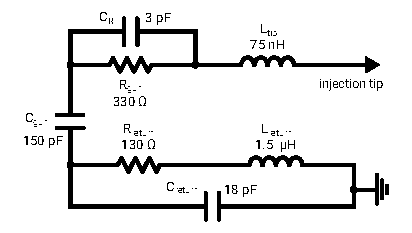
\includegraphics[width=0.7\textwidth]{src/1/figures/gun_model.pdf}
  \caption{modèle de pistolet ESD}
  \label{fig:esd-gun-model}
\end{figure}

% Explain the waveform
La forme d'onde est fournie dans la figure \ref{iec_pulse}.
Elle est définie pour une charge de 2\textOmega{}.
L'impulsion commence par un pic d'une largeur de $1ns$.
Il est suivi par une partie plus lente d'amplitude plus faible, mais qui dure plus longtemps (approximativement $200ns$).
Les niveaux de tensions peuvent atteindre 15 kV et de courant 30 A.

\begin{figure}[!h]
  \centering
  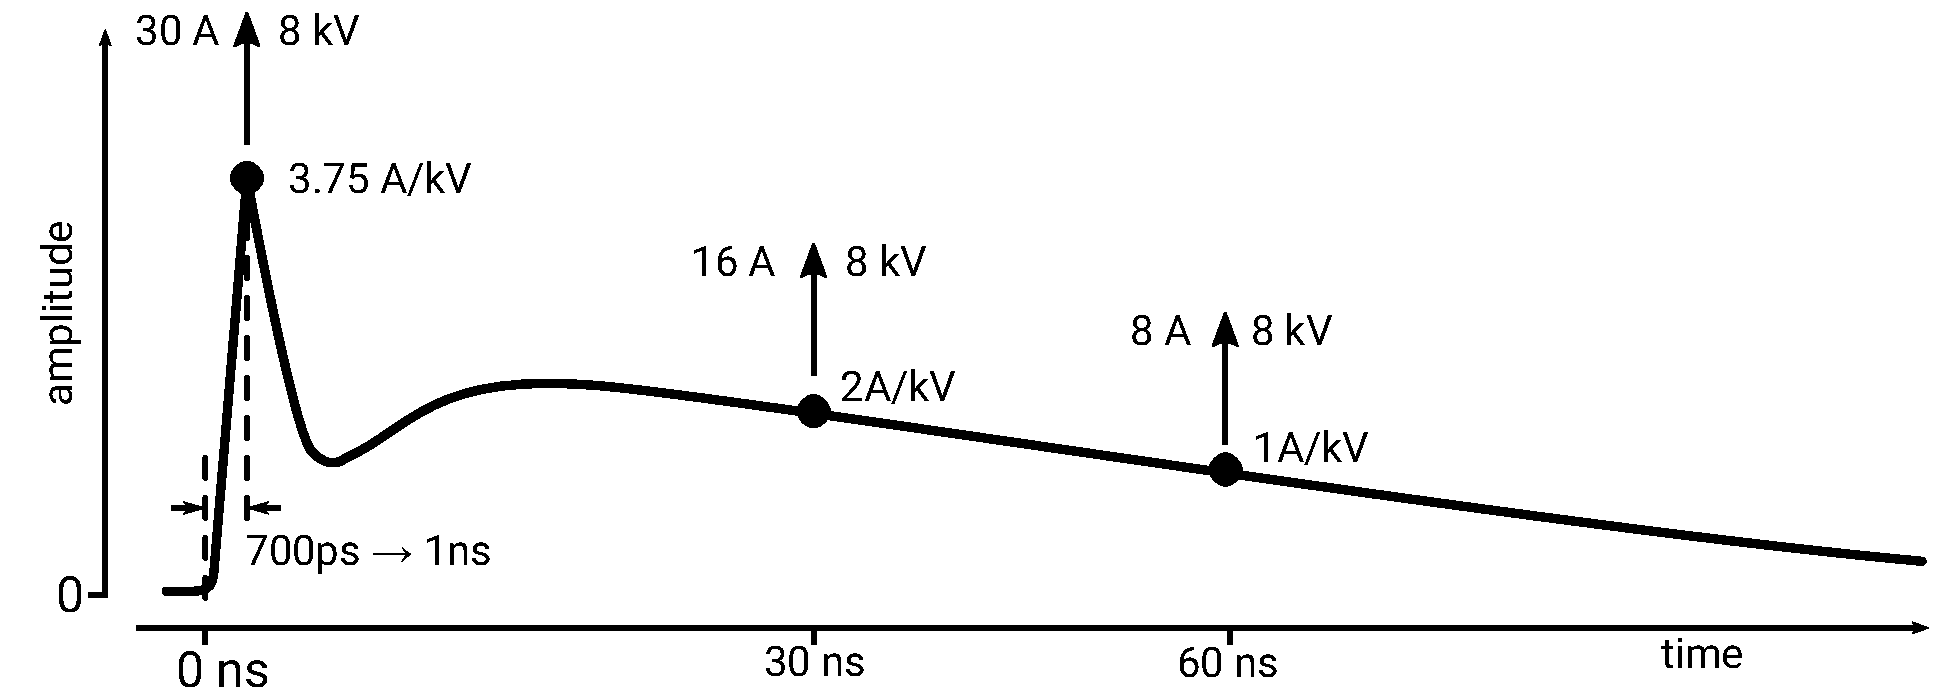
\includegraphics[width=\textwidth]{src/1/figures/iec61000-4-2_waveform.pdf}
  \caption{Propriétés d'une décharge IEC 61000-4-2 sur une résistance de 2\textOmega{}}
  \label{iec_pulse}
\end{figure}

% autres méthodes
Il existe un grand nombre d'autres méthodes de test, non spécifiques aux tests ESD mais qui peuvent permettre d'évaluer la robustesse des fonctions électroniques.
Dans l'automobile, le standard ISO 7637-2 est très largement employée pour qualifier les modules électroniques.
La méthode DPI (Direct Power Injection) est une méthode d'injection CEM très intéressante de par son circuit de couplage d'un stress sur une tension d'alimentation, qui est souvent nécessaire pour faire des tests ESD sur des produits en fonctionnement.

Une fois les produits testés, des cas de défaillances peuvent-être identifiés.
La partie suivante présente des cas de défaillances fonctionnelles trouvés dans la littérature.

\section{Méthodes d'analyse de faiblesses fonctionnelles}

Une revue de la littérature a permis d'identifier les études clés dans l'étude des circuits électroniques perturbés pendant leur fonctionnement par des ESD.
Certaines études concernent des cas de défaillance sur des circuits intégrés.
C'est le cas de l'étude de N. Lacrampe \cite{LacrampeTransientImmunity} sur des cœurs logiques en technologie CMOS 0.18 \textmu{}m exposés à des impulsions "very-fast" TLP.
Dans \cite{SDRAMCase}, des fautes fonctionnelles sont étudiées sur une mémoire de type SDRAM pendant son fonctionnement normal.
Deux types de défaillances de bus de communication vidéo sont présentés dans \cite{softFailSubsystem}.
Un scanner champ-proche a été utilisé sans succès pour tenter de localiser l'origine des défaillances.
Un affichage LCD (Liquid Crystal Display) est étudié dans \cite{softFailLCD}, présentant des problèmes d'affichages à la suite de décharges IEC 61000-4-2 \cite{iec61000-4-2}.
Malgré plusieurs tentatives à l'aide d'une injection champ proche et d'un TLP, les résultats furent infructueux et aucune piste ne put être identifiée comme point d'entrée de la décharge.
Une méthode d'investigation basée sur des simulations électromagnétiques est présentée dans \cite{softFailMobile} afin de déterminer les chemins de propagation de décharges causant des fautes sur un appareil mobile.
Une fois la cause défaillance déterminée, des réseaux de filtrage RC furent utilisés pour protéger les entrées et sorties physiques telles que les boutons et connecteurs.

% Case 1 - NXP bandgap + substrate coupling
Une cas d'étude typique de défaillance fonctionnelle est présenté par K. Abouda dans \cite{softfailEMCIC}.
L'étude concerne la perte de la régulation de tension assurée normalement dans un circuit intégré pour l'automobile, à la suite d'une décharge BCI (Bulk Current Injection) ISO11452-4 \cite{iso11452}.
Les chemins de propagation et de couplages à l'intérieur du circuit sont recherchés manuellement dans le design du produit, à l'aide de multiples simulations.
La cause de la défaillance a pu être identifiée avec succès et le design a été corrigé afin d'appliquer un filtrage adéquat directement sur le silicium pour éliminer le problème.

% Méthode injection
Plusieurs méthodes d'injection ont été utilisées au travers de toutes ces études.
La méthode DPI \cite{iec62132-4} a été utilisée plusieurs fois pour coupler un ESD sur une alimentation.
Une cellule TEM (Transverse Electro Magnetic) modifiée de dimensions réduites a également été proposée dans \cite{SDRAMCase}.
Une injection par champ proche fut employée dans \cite{softFailLCD} afin de tenter d'identifier le point d'entrée le plus susceptible des perturbations.
Un TLP couplé capacitivement fut également utilisé comme alternative à l'injection champ proche.

% Méthodes d'observation
Plusieurs approches de modélisation ont été proposées.
Elle se basent sur une large gamme de techniques allant de simulation 3D basées sur la physique des semi-conducteurs, jusqu'à des modèles boite-noire et comportementaux.
M. Scholz a publié une méthode de simulation ESD mixte dans \cite{mixedModeESDSims} qui combine des modèles SPICE et TCAD.
Dans \cite{usb2ESDProtection}, des caractérisations TLP sont utilisées comme modèles I(V) pour des protections ESD internes et externes.
Les paramètres S du la carte électroniques sont extraits avec un logiciel de simulation électromagnétique 3D.
Cette approche de modélisation s'est avérée fructueuse pour simuler les interactions entre des composants discrets et des composants intégrés sur silicium.
Une méthode de simulation 3D électromagnétique au niveau circuit intégré est également proposée par N. Lacrampe dans \cite{LacrampeTransientImmunity}.
Au niveau carte, les pistes métalliques sont modélisées avec un réseau RLC.
Le package est modélisé avec les informations contenues dans le modèle IBIS \cite{ibis-spec}.
Le générateur de stress, un TLP, est modélisé avec une table I(V), en série avec une résistance de 50\textOmega{}.
Dans \cite{softFailMobile}, des simulations électromagnétiques fullwave sont réalisées pour une analyse ESD en alimenté.
Des composants au niveau système sont simulés, tels que des coques en métal et des batteries.
La simulation 3D EM a permis d'identifier le chemin principal de propagation et de localiser le point de défaillance.

Globalement, ces études montrent qu'il est très complexe d'identifier la cause d'une défaillance fonctionnelle.
Il semble nécessaire d'avoir accès au design afin d'être capable de proposer des corrections efficaces.
La complexité des circuits intégrés est une grosse barrière pour déterminer la cause de défaillance, et des méthodes aussi bien de mesure que de simulation au niveau circuit-intégré sont donc requises.
